\subsection{Rodzaje grafów}
Graf skierowany to graf, w którym krawędzie są zorientowanymi parami wierzchołków.
Maksymalnie jedna krawędź może łączyć dwa wierzchołki w dowolnym kierunku.
Na ilustracji, linie łączące wierzchołki są oznaczone strzałkami.

\begin{figure}[ht]
	\centering
	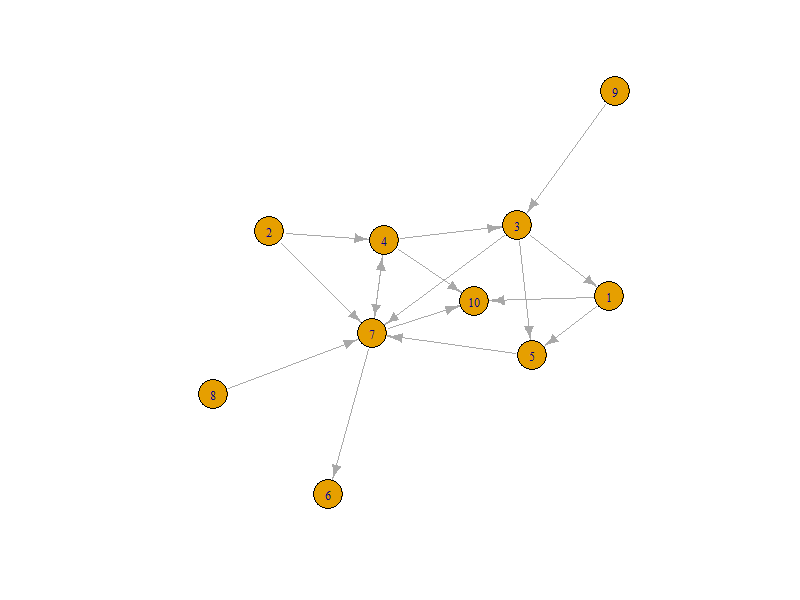
\includegraphics[height=11cm]{partials/images/graph_directed.png}
	\caption{Przykład grafu skierowanego}
\label{Fig:GraphUndirected}
\end{figure}

Graf nieskierowany to graf, w którym krawędzie nie mają kierunku.
Możemy mieć tylko jedną krawędź łączącą dwa wierzchołki (ponieważ V to zbiór).
Zwykle pętle w wierzchołkach nie są pożądane.
Wszystkie grafy są nieskierowane, chyba że zaznaczono inaczej.

\begin{figure}[ht]
	\centering
	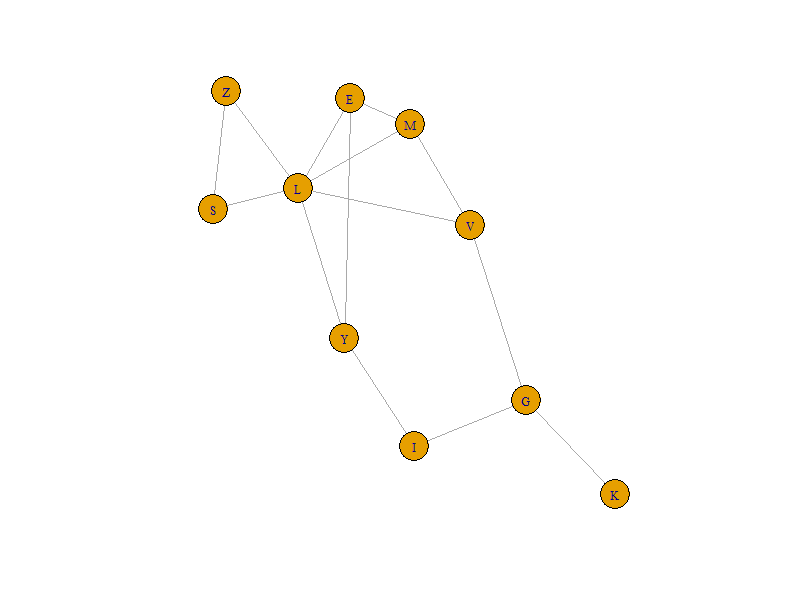
\includegraphics[height=11cm]{partials/images/graph_undirected.png}
	\caption{Przykład grafu nieskierowanego}
    \label{Fig:GraphDirected}
\end{figure}

\subsection{Rozpoznawanie grafów}
Lorem Ipsum is simply dummy text of the printing and typesetting industry. Lorem Ipsum has been the industry's standard dummy text ever since the 1500s, when an unknown printer took a galley of type and scrambled it to make a type specimen book. It has survived not only five centuries, but also the leap into electronic typesetting, remaining essentially unchanged. It was popularised in the 1960s with the release of Letraset sheets containing Lorem Ipsum passages, and more recently with desktop publishing software like Aldus PageMaker including versions of Lorem Ipsum.
